\documentclass{article}
\usepackage[utf8]{inputenc}
\usepackage{graphicx}
\usepackage{a4wide}
\usepackage{float}
\addtolength{\topmargin}{-1in}
\pagenumbering{gobble}

\title{Is Florida getting warmer?}
\author{Kate Griffin (kate.griffin21@imperial.ac.uk}
\date{November 2021}

\begin{document}
	
	\maketitle
	
	\section{Introduction}
	A permutation analysis was conducted to investigate whether Florida is getting warmer. The correlation between the temperature and year was calculated using data from the annual temperature dataset from Key West in Florida, USA for the 20th century. 
	
	\section{Methods}
	The Pearson's correlation coefficient between temperature and year was calculated. The temperature data was re-sampled to make 1000 permuted samples. The correlation coefficient was calculated between year and permuted temperature values. The fraction of permuted coefficients which were greater than the observed coefficient was calculated (i.e. the asymptotic p-value). The distribution of permuted samples were visualised on a histogram, with a vertical line representing the observed correlation coefficient. 
	
	\section{Results} 
	There was a significant correlation between temperature and year (p-value=0). 
	\begin{figure}[H]
		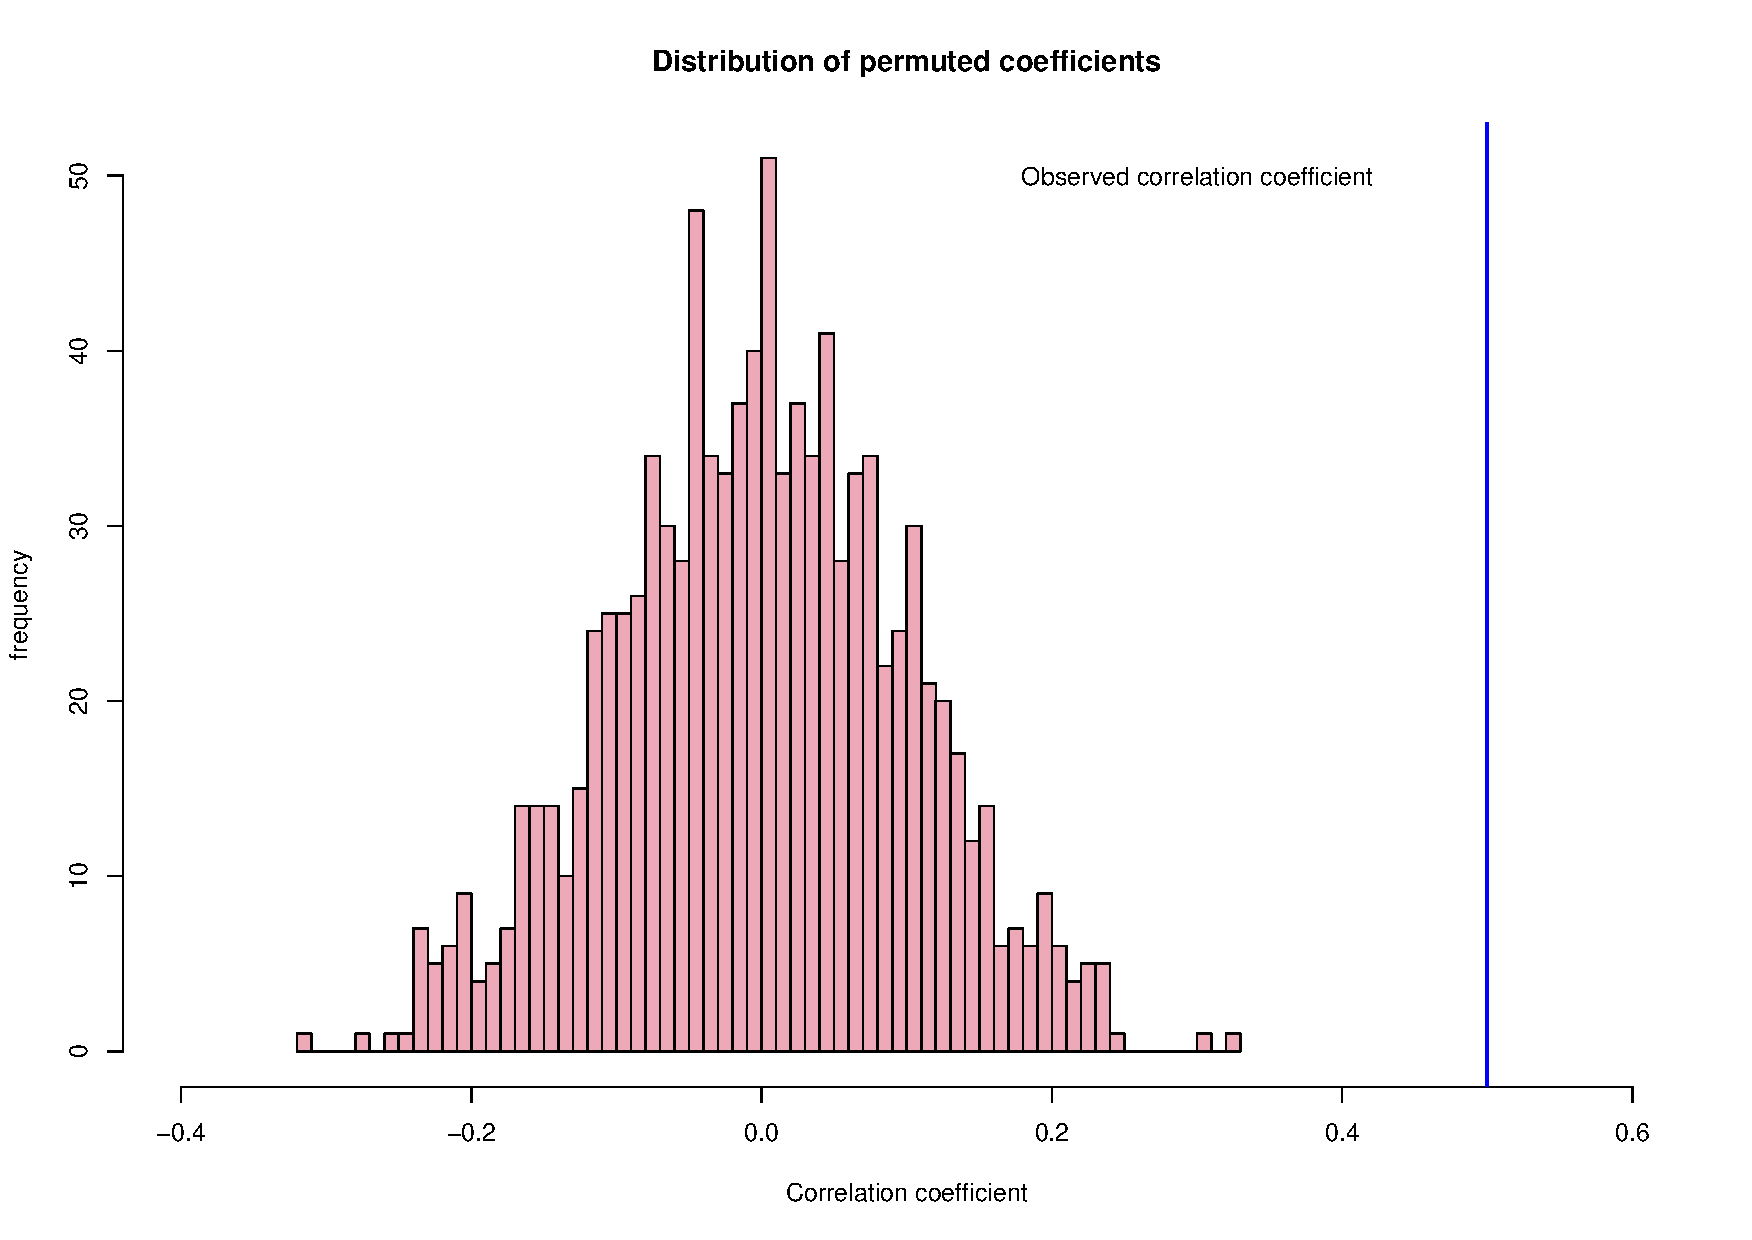
\includegraphics[scale=0.4]{../results/Florida_hist.pdf}
		\caption{The distribution of correlation coefficients of permuted samples. The blue line represents the observed coefficient.1}
		\label{The distribution of correlation coefficients of permuted samples. The blue line represents the observed coefficient.1}
	\end{figure}
	
\end{document}